We seek to resolve the issues of non-uniqueness by employing mixed strategies. 
% By granting each agent several possible trajectories within the dynamic constraints, each agent may compute the possible   
We first define a reference trajectory for the evading spacecraft. 
We determine the state at discrete points around the reference orbit
To approximate the orbit bandwidth, we define the cross-section of the orbit to be a hexagon.
To play the pursuit evasion game, the evading spacecraft will target one of the vertices of the hexagon at a future point of the orbit.

To lift the pursuit evasion game from the planar environment to a 3-dimensional game subject to orbital dynamics constraints, a local reference frame for a 6-sided polygon was first defined. The polygon is centered along the reference trajectory. 

\begin{figure*}[t] % [t] pulls it to the top of the page
    \centering
    \begin{subfigure}[b]{0.31\textwidth}
        \centering
        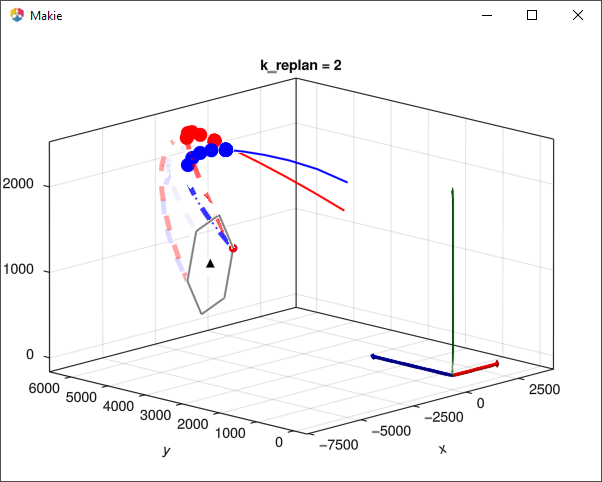
\includegraphics[width=\textwidth]{images/k_replan_1.png}
        \caption{Second replanning period.}
        \label{fig:first}
    \end{subfigure}
    % \hfill % Adds horizontal space between the two images
    \begin{subfigure}[b]{0.31\textwidth}
        \centering
        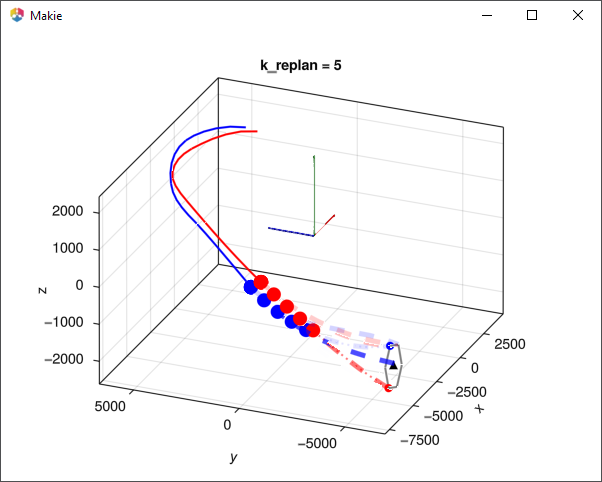
\includegraphics[width=\textwidth]{images/k_replan_5.png}
        \caption{Fifth replanning period.}
        \label{fig:second}
    \end{subfigure}
    \begin{subfigure}[b]{0.31\textwidth}
        \centering 
        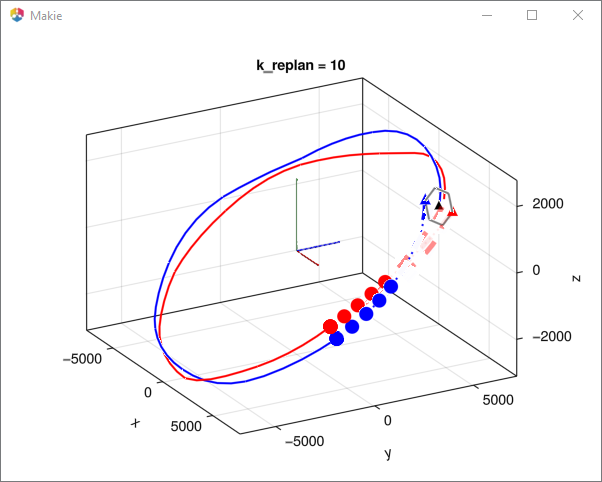
\includegraphics[width=\textwidth]{images/k_replan_10.png}
        \caption{Tenth (and final) replanning period.} 
    \end{subfigure}
    \caption{\textbf{Propagated and mixed trajectories at the the 2nd, 5th, and 10th replanning periods.} The solid lines represent the trajectories already traveled during past planning periods. For the current planning period, the dots represent the propagated (and chosen) trajectories, and the dashed lines represent the candidate trajectories. The darkness of the dashed lines represent the weights associated with each trajectory. }
    \label{fig:main_figure}
\end{figure*}

Then, we compute trajectories targeting the 6 vertices of the polygon for the pursuer and the evader. 
The stage cost at each time instant was computed and then averaged along the entire trajectory. 
\begin{equation}
    c(t) = \sqrt{ || \mathbf{r}_1(t) - \mathbf{r}_2(t) ||_2 + \lambda_1 } + \lambda_2 ( || \mathbf{u}_1(t) ||_2 - || \mathbf{u}_2(t) ||_2 )
\end{equation} 
The average stage cost was then saved in a cost matrix for each trajectory / vertex pairing. This results in a 6x6 cost matrix for each player. 

We are playing a zero sum game, so the cost matrix for one player is equivalent to the negative of the cost matrix for the other player. 

To solve the mixed strategy problem and find weights for each trajectory, we first transform the game to ensure that the cost matrix is entrywise positive. 

Then, we solve the simplex linear program associated with a zero sum game. 
% 
\begin{align}
    \max_{ \mathbf{z} \in \mathbb{R}^6 }    & \; \; \mathbf{1}^T \mathbf{z} \\ 
    \text{ subject to }                     & \; \; \mathbf{1} \geq A^T \mathbf{z}    
\end{align} 

Finally, we transform the solution into a probability simplex. This results in mixing weights $ x^* $ for each trajectory / vertex for each player. 

\begin{equation}
    x^* = \frac{\mathbf{z^*}}{ \mathbf{1}^T \mathbf{z^*} }  
\end{equation} 

To play the game, we sample from the mixing weights for each player. To construct the initial guess for the control input, we compute the initial velocity vector required for a Lambert transfer. We divide the velocity into 10 segments for each planning period of the trajectory to set as the initial guess vector. 

% \begin{figure*}[!t]
%     \centering
%     \begin{subfigure}{0.48\linewidth}
%         \centering
%         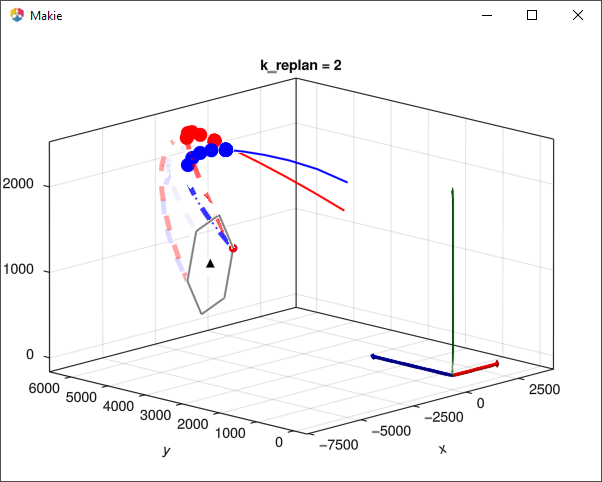
\includegraphics[width=\linewidth]{images/k_replan_1.png}
%         \caption{Body rates $\omega_{body}$ (rad/s) }
%         \label{fig:omega_bus} 
%     \end{subfigure}
%     \hfill
%     \begin{subfigure}{0.48\linewidth}
%         \centering
%         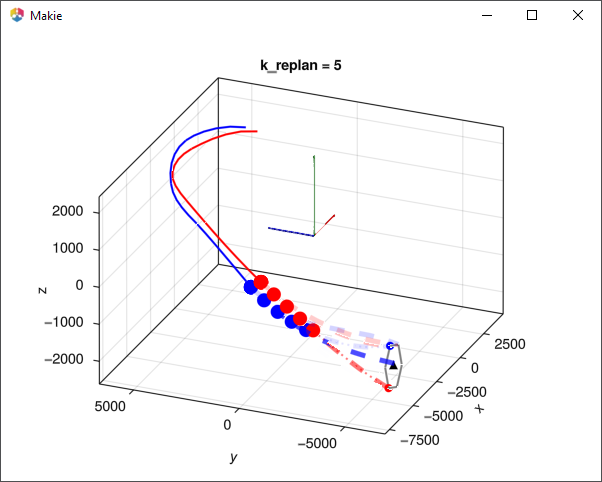
\includegraphics[width=\linewidth]{images/k_replan_5.png}
%         \caption{Body rates $\omega_{body}$ FFT }
%         \label{fig:omega_bus_fft} 
%     \end{subfigure}
%     \caption{asdf} 
%     \label{fig:cgs_rigid_body} 
%     \vspace{-1em}
% \end{figure*}

\begin{equation}
    \boldsymbol{v}_1, \boldsymbol{v}_2 = 
    % minLambert
    \operatorname{Lambert}
    (\boldsymbol{r}^P_0, \boldsymbol{r}^E_0, t_2, t_1, \mu). \label{eq:min_lambert}
\end{equation} 

\begin{figure}[ht!]
    \centering
    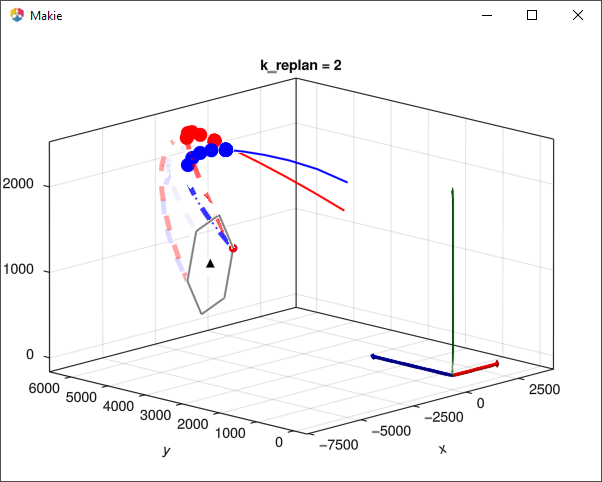
\includegraphics[width=0.9\linewidth]{images/k_replan_1.png}
    \caption{Caption}
    \label{fig:enter-label}
\end{figure}

% \begin{figure}[ht!]
%     \centering
%     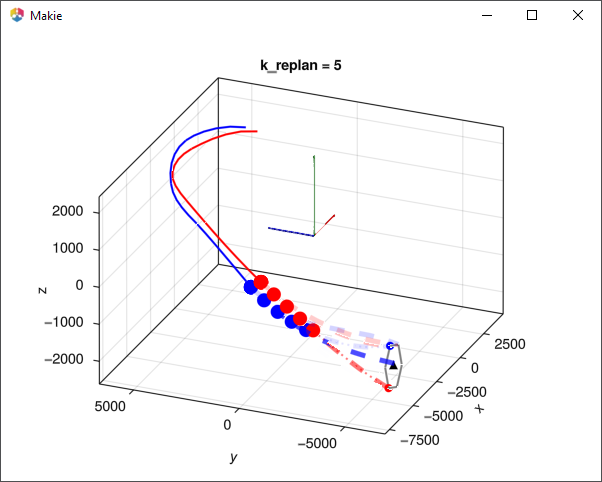
\includegraphics[width=0.9\linewidth]{images/k_replan_5.png}
%     \caption{Caption}
%     \label{fig:enter-label}
% \end{figure}

% \begin{figure}[ht!]
%     \centering
%     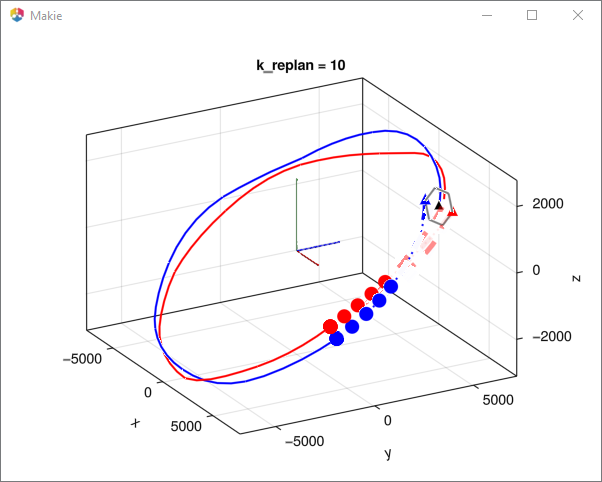
\includegraphics[width=0.9\linewidth]{images/k_replan_10.png}
%     \caption{Caption}
%     \label{fig:enter-label}
% \end{figure}





